\documentclass{standalone}
\usepackage{tikz}
\usetikzlibrary{patterns, positioning}


\begin{document}
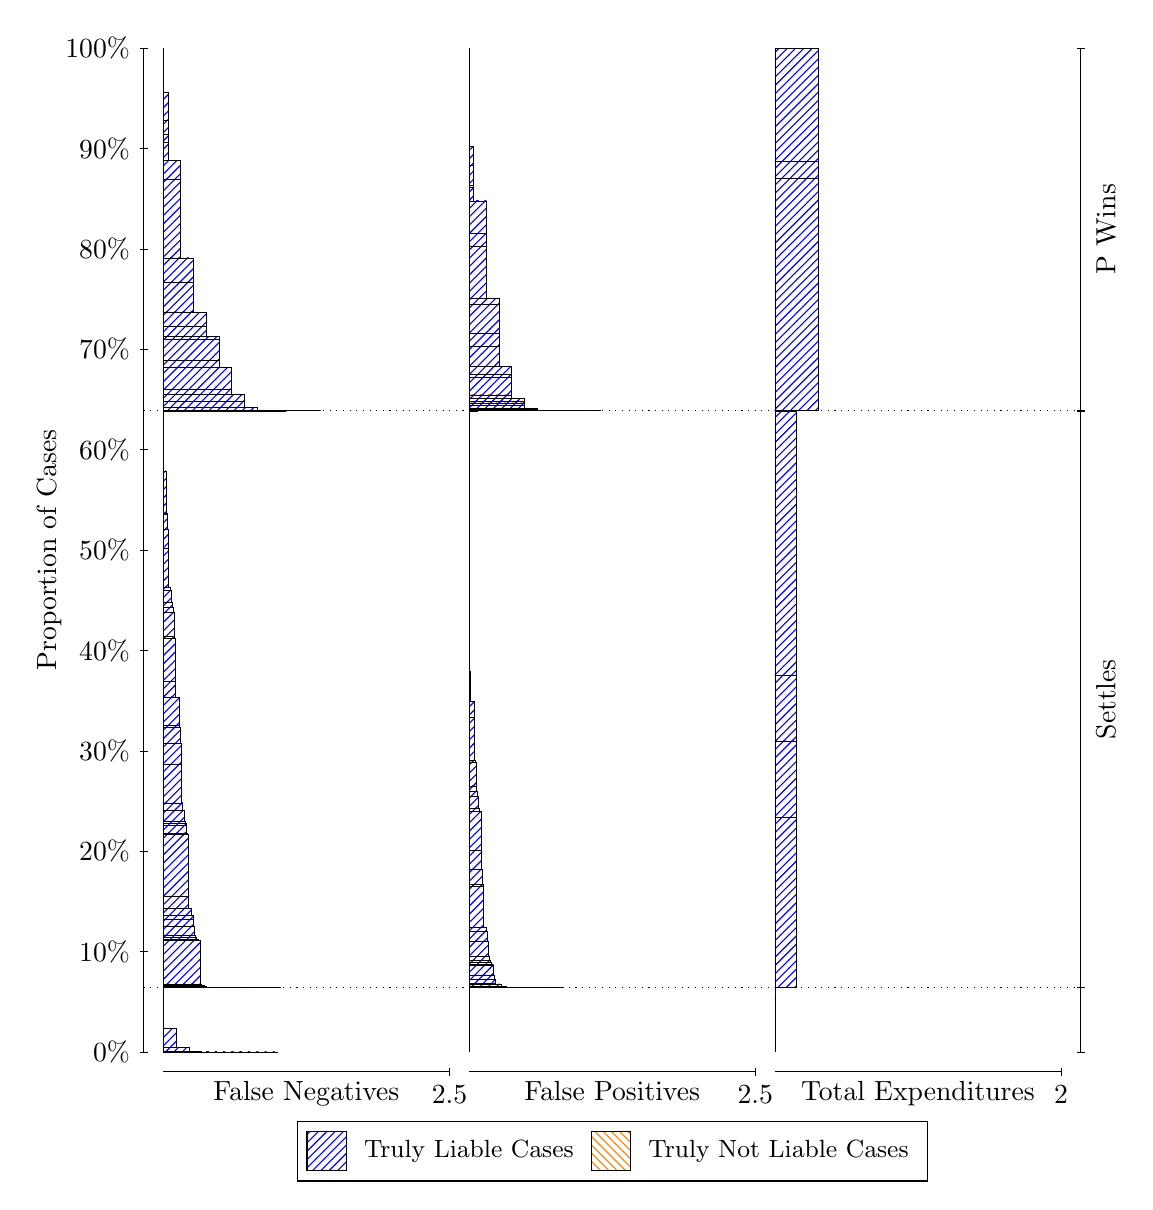
\begin{tikzpicture}
\draw[black, very thin] (1.5,1.75) -- (1.5,14.5);
\node[rotate=90, text=black, anchor=center] at (0.3, 8.125) {Proportion of Cases};
\draw[black, very thin] (1.45,1.75) -- (1.55,1.75);
\node[text=black, anchor=east] at (1.45, 1.75) {0\%};
\draw[black, very thin] (1.45,3.025) -- (1.55,3.025);
\node[text=black, anchor=east] at (1.45, 3.025) {10\%};
\draw[black, very thin] (1.45,4.3) -- (1.55,4.3);
\node[text=black, anchor=east] at (1.45, 4.3) {20\%};
\draw[black, very thin] (1.45,5.575) -- (1.55,5.575);
\node[text=black, anchor=east] at (1.45, 5.575) {30\%};
\draw[black, very thin] (1.45,6.85) -- (1.55,6.85);
\node[text=black, anchor=east] at (1.45, 6.85) {40\%};
\draw[black, very thin] (1.45,8.125) -- (1.55,8.125);
\node[text=black, anchor=east] at (1.45, 8.125) {50\%};
\draw[black, very thin] (1.45,9.4) -- (1.55,9.4);
\node[text=black, anchor=east] at (1.45, 9.4) {60\%};
\draw[black, very thin] (1.45,10.675) -- (1.55,10.675);
\node[text=black, anchor=east] at (1.45, 10.675) {70\%};
\draw[black, very thin] (1.45,11.95) -- (1.55,11.95);
\node[text=black, anchor=east] at (1.45, 11.95) {80\%};
\draw[black, very thin] (1.45,13.225) -- (1.55,13.225);
\node[text=black, anchor=east] at (1.45, 13.225) {90\%};
\draw[black, very thin] (1.45,14.5) -- (1.55,14.5);
\node[text=black, anchor=east] at (1.45, 14.5) {100\%};

\draw[black, very thin] (13.4,1.75) -- (13.4,14.5);
\draw[black, very thin] (13.35,1.75) -- (13.45,1.75);
\node[anchor=west] at (13.35, 1.75) {};
\draw[black, very thin] (13.35,2.5655) -- (13.45,2.5655);
\node[anchor=west] at (13.35, 2.5655) {};
\draw[black, very thin] (13.35,9.8923) -- (13.45,9.8923);
\node[anchor=west] at (13.35, 9.8923) {};
\draw[black, very thin] (13.35,9.8952) -- (13.45,9.8952);
\node[anchor=west] at (13.35, 9.8952) {};
\draw[black, very thin] (13.35,14.5) -- (13.45,14.5);
\node[anchor=west] at (13.35, 14.5) {};

\draw[black, very thin, pattern color=blue, pattern=north east lines] (1.75,1.75) rectangle (3.2033,1.75);
\draw[black, very thin, pattern color=blue, pattern=north east lines] (1.75,1.75) rectangle (3.0419,1.75);
\draw[black, very thin, pattern color=blue, pattern=north east lines] (1.75,1.75) rectangle (2.8804,1.75);
\draw[black, very thin, pattern color=blue, pattern=north east lines] (1.75,1.75) rectangle (2.7189,1.75);
\draw[black, very thin, pattern color=blue, pattern=north east lines] (1.75,1.75) rectangle (2.5574,1.75);
\draw[black, very thin, pattern color=blue, pattern=north east lines] (1.75,1.75) rectangle (2.3959,1.7502);
\draw[black, very thin, pattern color=blue, pattern=north east lines] (1.75,1.7502) rectangle (2.2344,1.7558);
\draw[black, very thin, pattern color=blue, pattern=north east lines] (1.75,1.7558) rectangle (2.073,1.8123);
\draw[black, very thin, pattern color=blue, pattern=north east lines] (1.75,1.8123) rectangle (1.9115,2.0523);
\draw[black, very thin, pattern color=orange, pattern=north west lines] (1.75,2.0523) rectangle (1.75,2.0523);
\draw[black, very thin, pattern color=blue, pattern=north east lines] (1.75,2.0523) rectangle (1.75,2.5655);
\draw[black, very thin, pattern color=blue, pattern=north east lines] (1.75,2.5655) rectangle (3.2397,2.5655);
\draw[black, very thin, pattern color=blue, pattern=north east lines] (1.75,2.5655) rectangle (3.167,2.5655);
\draw[black, very thin, pattern color=blue, pattern=north east lines] (1.75,2.5655) rectangle (3.0943,2.5655);
\draw[black, very thin, pattern color=blue, pattern=north east lines] (1.75,2.5655) rectangle (3.0782,2.5655);
\draw[black, very thin, pattern color=blue, pattern=north east lines] (1.75,2.5655) rectangle (3.0217,2.5655);
\draw[black, very thin, pattern color=blue, pattern=north east lines] (1.75,2.5655) rectangle (3.0055,2.5655);
\draw[black, very thin, pattern color=blue, pattern=north east lines] (1.75,2.5655) rectangle (2.949,2.5655);
\draw[black, very thin, pattern color=blue, pattern=north east lines] (1.75,2.5655) rectangle (2.9329,2.5655);
\draw[black, very thin, pattern color=blue, pattern=north east lines] (1.75,2.5655) rectangle (2.9167,2.5655);
\draw[black, very thin, pattern color=blue, pattern=north east lines] (1.75,2.5655) rectangle (2.8763,2.5655);
\draw[black, very thin, pattern color=blue, pattern=north east lines] (1.75,2.5655) rectangle (2.8602,2.5655);
\draw[black, very thin, pattern color=blue, pattern=north east lines] (1.75,2.5655) rectangle (2.844,2.5655);
\draw[black, very thin, pattern color=blue, pattern=north east lines] (1.75,2.5655) rectangle (2.8037,2.5655);
\draw[black, very thin, pattern color=blue, pattern=north east lines] (1.75,2.5655) rectangle (2.8037,2.5655);
\draw[black, very thin, pattern color=blue, pattern=north east lines] (1.75,2.5655) rectangle (2.7875,2.5655);
\draw[black, very thin, pattern color=blue, pattern=north east lines] (1.75,2.5655) rectangle (2.7714,2.5655);
\draw[black, very thin, pattern color=blue, pattern=north east lines] (1.75,2.5655) rectangle (2.7552,2.5655);
\draw[black, very thin, pattern color=blue, pattern=north east lines] (1.75,2.5655) rectangle (2.731,2.5655);
\draw[black, very thin, pattern color=blue, pattern=north east lines] (1.75,2.5655) rectangle (2.7149,2.5655);
\draw[black, very thin, pattern color=blue, pattern=north east lines] (1.75,2.5655) rectangle (2.6987,2.5655);
\draw[black, very thin, pattern color=blue, pattern=north east lines] (1.75,2.5655) rectangle (2.6826,2.5655);
\draw[black, very thin, pattern color=blue, pattern=north east lines] (1.75,2.5655) rectangle (2.6583,2.5655);
\draw[black, very thin, pattern color=blue, pattern=north east lines] (1.75,2.5655) rectangle (2.6422,2.5655);
\draw[black, very thin, pattern color=blue, pattern=north east lines] (1.75,2.5655) rectangle (2.6422,2.5655);
\draw[black, very thin, pattern color=blue, pattern=north east lines] (1.75,2.5655) rectangle (2.626,2.5655);
\draw[black, very thin, pattern color=blue, pattern=north east lines] (1.75,2.5655) rectangle (2.6099,2.5655);
\draw[black, very thin, pattern color=blue, pattern=north east lines] (1.75,2.5655) rectangle (2.5937,2.5655);
\draw[black, very thin, pattern color=blue, pattern=north east lines] (1.75,2.5655) rectangle (2.5857,2.5655);
\draw[black, very thin, pattern color=blue, pattern=north east lines] (1.75,2.5655) rectangle (2.5695,2.5655);
\draw[black, very thin, pattern color=blue, pattern=north east lines] (1.75,2.5655) rectangle (2.5534,2.5655);
\draw[black, very thin, pattern color=blue, pattern=north east lines] (1.75,2.5655) rectangle (2.5372,2.5655);
\draw[black, very thin, pattern color=blue, pattern=north east lines] (1.75,2.5655) rectangle (2.5211,2.5655);
\draw[black, very thin, pattern color=blue, pattern=north east lines] (1.75,2.5655) rectangle (2.513,2.5655);
\draw[black, very thin, pattern color=blue, pattern=north east lines] (1.75,2.5655) rectangle (2.4969,2.5655);
\draw[black, very thin, pattern color=blue, pattern=north east lines] (1.75,2.5655) rectangle (2.4807,2.5655);
\draw[black, very thin, pattern color=blue, pattern=north east lines] (1.75,2.5655) rectangle (2.4646,2.5655);
\draw[black, very thin, pattern color=blue, pattern=north east lines] (1.75,2.5655) rectangle (2.4484,2.5656);
\draw[black, very thin, pattern color=blue, pattern=north east lines] (1.75,2.5656) rectangle (2.4403,2.5656);
\draw[black, very thin, pattern color=blue, pattern=north east lines] (1.75,2.5656) rectangle (2.4323,2.5656);
\draw[black, very thin, pattern color=blue, pattern=north east lines] (1.75,2.5656) rectangle (2.4242,2.5656);
\draw[black, very thin, pattern color=blue, pattern=north east lines] (1.75,2.5656) rectangle (2.408,2.5656);
\draw[black, very thin, pattern color=blue, pattern=north east lines] (1.75,2.5656) rectangle (2.3919,2.5661);
\draw[black, very thin, pattern color=blue, pattern=north east lines] (1.75,2.5661) rectangle (2.3757,2.5662);
\draw[black, very thin, pattern color=blue, pattern=north east lines] (1.75,2.5662) rectangle (2.3677,2.5663);
\draw[black, very thin, pattern color=blue, pattern=north east lines] (1.75,2.5663) rectangle (2.3596,2.5663);
\draw[black, very thin, pattern color=blue, pattern=north east lines] (1.75,2.5663) rectangle (2.3515,2.5663);
\draw[black, very thin, pattern color=blue, pattern=north east lines] (1.75,2.5663) rectangle (2.3354,2.5669);
\draw[black, very thin, pattern color=blue, pattern=north east lines] (1.75,2.5669) rectangle (2.3192,2.5688);
\draw[black, very thin, pattern color=blue, pattern=north east lines] (1.75,2.5688) rectangle (2.3192,2.5688);
\draw[black, very thin, pattern color=blue, pattern=north east lines] (1.75,2.5688) rectangle (2.3031,2.5745);
\draw[black, very thin, pattern color=blue, pattern=north east lines] (1.75,2.5745) rectangle (2.295,2.5858);
\draw[black, very thin, pattern color=blue, pattern=north east lines] (1.75,2.5858) rectangle (2.2869,2.5881);
\draw[black, very thin, pattern color=blue, pattern=north east lines] (1.75,2.5881) rectangle (2.2789,2.5884);
\draw[black, very thin, pattern color=blue, pattern=north east lines] (1.75,2.5884) rectangle (2.2708,2.5927);
\draw[black, very thin, pattern color=blue, pattern=north east lines] (1.75,2.5927) rectangle (2.2627,2.5929);
\draw[black, very thin, pattern color=blue, pattern=north east lines] (1.75,2.5929) rectangle (2.2466,2.5929);
\draw[black, very thin, pattern color=blue, pattern=north east lines] (1.75,2.5929) rectangle (2.2304,2.6134);
\draw[black, very thin, pattern color=blue, pattern=north east lines] (1.75,2.6134) rectangle (2.2223,3.1659);
\draw[black, very thin, pattern color=blue, pattern=north east lines] (1.75,3.1659) rectangle (2.2143,3.1689);
\draw[black, very thin, pattern color=blue, pattern=north east lines] (1.75,3.1689) rectangle (2.2062,3.1748);
\draw[black, very thin, pattern color=blue, pattern=north east lines] (1.75,3.1748) rectangle (2.1981,3.1769);
\draw[black, very thin, pattern color=blue, pattern=north east lines] (1.75,3.1769) rectangle (2.19,3.1788);
\draw[black, very thin, pattern color=blue, pattern=north east lines] (1.75,3.1788) rectangle (2.1739,3.2005);
\draw[black, very thin, pattern color=blue, pattern=north east lines] (1.75,3.2005) rectangle (2.1577,3.233);
\draw[black, very thin, pattern color=blue, pattern=north east lines] (1.75,3.233) rectangle (2.1577,3.2331);
\draw[black, very thin, pattern color=blue, pattern=north east lines] (1.75,3.2331) rectangle (2.1416,3.35);
\draw[black, very thin, pattern color=blue, pattern=north east lines] (1.75,3.35) rectangle (2.1335,3.4345);
\draw[black, very thin, pattern color=blue, pattern=north east lines] (1.75,3.4345) rectangle (2.1254,3.4827);
\draw[black, very thin, pattern color=blue, pattern=north east lines] (1.75,3.4827) rectangle (2.1174,3.488);
\draw[black, very thin, pattern color=blue, pattern=north east lines] (1.75,3.488) rectangle (2.1093,3.5719);
\draw[black, very thin, pattern color=blue, pattern=north east lines] (1.75,3.5719) rectangle (2.1012,3.5744);
\draw[black, very thin, pattern color=blue, pattern=north east lines] (1.75,3.5744) rectangle (2.0851,3.5744);
\draw[black, very thin, pattern color=blue, pattern=north east lines] (1.75,3.5744) rectangle (2.0689,3.722);
\draw[black, very thin, pattern color=blue, pattern=north east lines] (1.75,3.722) rectangle (2.0609,4.5144);
\draw[black, very thin, pattern color=blue, pattern=north east lines] (1.75,4.5144) rectangle (2.0528,4.5335);
\draw[black, very thin, pattern color=blue, pattern=north east lines] (1.75,4.5335) rectangle (2.0447,4.6279);
\draw[black, very thin, pattern color=blue, pattern=north east lines] (1.75,4.6279) rectangle (2.0366,4.6524);
\draw[black, very thin, pattern color=blue, pattern=north east lines] (1.75,4.6524) rectangle (2.0286,4.682);
\draw[black, very thin, pattern color=blue, pattern=north east lines] (1.75,4.682) rectangle (2.0124,4.8206);
\draw[black, very thin, pattern color=blue, pattern=north east lines] (1.75,4.8206) rectangle (1.9963,4.9137);
\draw[black, very thin, pattern color=blue, pattern=north east lines] (1.75,4.9137) rectangle (1.9963,4.9142);
\draw[black, very thin, pattern color=blue, pattern=north east lines] (1.75,4.9142) rectangle (1.9801,5.4048);
\draw[black, very thin, pattern color=blue, pattern=north east lines] (1.75,5.4048) rectangle (1.972,5.6723);
\draw[black, very thin, pattern color=blue, pattern=north east lines] (1.75,5.6723) rectangle (1.964,5.872);
\draw[black, very thin, pattern color=blue, pattern=north east lines] (1.75,5.872) rectangle (1.9559,5.8958);
\draw[black, very thin, pattern color=blue, pattern=north east lines] (1.75,5.8958) rectangle (1.9478,6.2535);
\draw[black, very thin, pattern color=blue, pattern=north east lines] (1.75,6.2535) rectangle (1.9397,6.2592);
\draw[black, very thin, pattern color=blue, pattern=north east lines] (1.75,6.2592) rectangle (1.9236,6.2592);
\draw[black, very thin, pattern color=blue, pattern=north east lines] (1.75,6.2592) rectangle (1.9074,6.4519);
\draw[black, very thin, pattern color=blue, pattern=north east lines] (1.75,6.4519) rectangle (1.8994,7.0045);
\draw[black, very thin, pattern color=blue, pattern=north east lines] (1.75,7.0045) rectangle (1.8913,7.0247);
\draw[black, very thin, pattern color=blue, pattern=north east lines] (1.75,7.0247) rectangle (1.8832,7.3298);
\draw[black, very thin, pattern color=blue, pattern=north east lines] (1.75,7.3298) rectangle (1.8751,7.3914);
\draw[black, very thin, pattern color=blue, pattern=north east lines] (1.75,7.3914) rectangle (1.8671,7.4659);
\draw[black, very thin, pattern color=blue, pattern=north east lines] (1.75,7.4659) rectangle (1.8509,7.6073);
\draw[black, very thin, pattern color=blue, pattern=north east lines] (1.75,7.6073) rectangle (1.8348,7.6556);
\draw[black, very thin, pattern color=blue, pattern=north east lines] (1.75,7.6556) rectangle (1.8348,7.6561);
\draw[black, very thin, pattern color=blue, pattern=north east lines] (1.75,7.6561) rectangle (1.8186,8.1431);
\draw[black, very thin, pattern color=blue, pattern=north east lines] (1.75,8.1431) rectangle (1.8106,8.3888);
\draw[black, very thin, pattern color=blue, pattern=north east lines] (1.75,8.3888) rectangle (1.8025,8.577);
\draw[black, very thin, pattern color=blue, pattern=north east lines] (1.75,8.577) rectangle (1.7944,8.5976);
\draw[black, very thin, pattern color=blue, pattern=north east lines] (1.75,8.5976) rectangle (1.7863,9.1273);
\draw[black, very thin, pattern color=blue, pattern=north east lines] (1.75,9.1273) rectangle (1.7783,9.1297);
\draw[black, very thin, pattern color=blue, pattern=north east lines] (1.75,9.1297) rectangle (1.7621,9.1297);
\draw[black, very thin, pattern color=orange, pattern=north west lines] (1.75,9.1297) rectangle (1.75,9.1297);
\draw[black, very thin, pattern color=blue, pattern=north east lines] (1.75,9.1297) rectangle (1.75,9.8923);
\draw[black, very thin, pattern color=blue, pattern=north east lines] (1.75,9.8923) rectangle (3.3123,9.8923);
\draw[black, very thin, pattern color=blue, pattern=north east lines] (1.75,9.8923) rectangle (3.1509,9.8923);
\draw[black, very thin, pattern color=blue, pattern=north east lines] (1.75,9.8923) rectangle (2.9894,9.8923);
\draw[black, very thin, pattern color=blue, pattern=north east lines] (1.75,9.8923) rectangle (2.8279,9.8923);
\draw[black, very thin, pattern color=blue, pattern=north east lines] (1.75,9.8923) rectangle (2.6664,9.8923);
\draw[black, very thin, pattern color=blue, pattern=north east lines] (1.75,9.8923) rectangle (2.5049,9.8923);
\draw[black, very thin, pattern color=blue, pattern=north east lines] (1.75,9.8923) rectangle (2.3434,9.8923);
\draw[black, very thin, pattern color=blue, pattern=north east lines] (1.75,9.8923) rectangle (2.182,9.8927);
\draw[black, very thin, pattern color=blue, pattern=north east lines] (1.75,9.8927) rectangle (2.0205,9.8939);
\draw[black, very thin, pattern color=blue, pattern=north east lines] (1.75,9.8939) rectangle (1.859,9.8952);
\draw[black, very thin, pattern color=orange, pattern=north west lines] (1.75,9.8952) rectangle (1.75,9.8952);
\draw[black, very thin, pattern color=blue, pattern=north east lines] (1.75,9.8952) rectangle (3.7483,9.8952);
\draw[black, very thin, pattern color=blue, pattern=north east lines] (1.75,9.8952) rectangle (3.5869,9.8952);
\draw[black, very thin, pattern color=blue, pattern=north east lines] (1.75,9.8952) rectangle (3.4254,9.8952);
\draw[black, very thin, pattern color=blue, pattern=north east lines] (1.75,9.8952) rectangle (3.2639,9.8954);
\draw[black, very thin, pattern color=blue, pattern=north east lines] (1.75,9.8954) rectangle (3.2639,9.8955);
\draw[black, very thin, pattern color=blue, pattern=north east lines] (1.75,9.8955) rectangle (3.2599,9.8955);
\draw[black, very thin, pattern color=blue, pattern=north east lines] (1.75,9.8955) rectangle (3.1024,9.8994);
\draw[black, very thin, pattern color=blue, pattern=north east lines] (1.75,9.8994) rectangle (3.0984,9.8994);
\draw[black, very thin, pattern color=blue, pattern=north east lines] (1.75,9.8994) rectangle (3.0984,9.8994);
\draw[black, very thin, pattern color=blue, pattern=north east lines] (1.75,9.8994) rectangle (2.9409,9.9327);
\draw[black, very thin, pattern color=blue, pattern=north east lines] (1.75,9.9327) rectangle (2.9369,9.9327);
\draw[black, very thin, pattern color=blue, pattern=north east lines] (1.75,9.9327) rectangle (2.7794,10.016);
\draw[black, very thin, pattern color=blue, pattern=north east lines] (1.75,10.016) rectangle (2.7794,10.097);
\draw[black, very thin, pattern color=blue, pattern=north east lines] (1.75,10.097) rectangle (2.7754,10.097);
\draw[black, very thin, pattern color=blue, pattern=north east lines] (1.75,10.097) rectangle (2.7754,10.097);
\draw[black, very thin, pattern color=blue, pattern=north east lines] (1.75,10.097) rectangle (2.618,10.169);
\draw[black, very thin, pattern color=blue, pattern=north east lines] (1.75,10.169) rectangle (2.618,10.449);
\draw[black, very thin, pattern color=blue, pattern=north east lines] (1.75,10.449) rectangle (2.6139,10.449);
\draw[black, very thin, pattern color=blue, pattern=north east lines] (1.75,10.449) rectangle (2.4565,10.537);
\draw[black, very thin, pattern color=blue, pattern=north east lines] (1.75,10.537) rectangle (2.4565,10.801);
\draw[black, very thin, pattern color=blue, pattern=north east lines] (1.75,10.801) rectangle (2.4565,10.833);
\draw[black, very thin, pattern color=blue, pattern=north east lines] (1.75,10.833) rectangle (2.4524,10.834);
\draw[black, very thin, pattern color=blue, pattern=north east lines] (1.75,10.834) rectangle (2.4524,10.835);
\draw[black, very thin, pattern color=blue, pattern=north east lines] (1.75,10.835) rectangle (2.295,10.969);
\draw[black, very thin, pattern color=blue, pattern=north east lines] (1.75,10.969) rectangle (2.291,11.142);
\draw[black, very thin, pattern color=blue, pattern=north east lines] (1.75,11.142) rectangle (2.1335,11.142);
\draw[black, very thin, pattern color=blue, pattern=north east lines] (1.75,11.142) rectangle (2.1335,11.148);
\draw[black, very thin, pattern color=blue, pattern=north east lines] (1.75,11.148) rectangle (2.1335,11.148);
\draw[black, very thin, pattern color=blue, pattern=north east lines] (1.75,11.148) rectangle (2.1295,11.529);
\draw[black, very thin, pattern color=blue, pattern=north east lines] (1.75,11.529) rectangle (2.1295,11.836);
\draw[black, very thin, pattern color=blue, pattern=north east lines] (1.75,11.836) rectangle (1.972,11.836);
\draw[black, very thin, pattern color=blue, pattern=north east lines] (1.75,11.836) rectangle (1.972,11.836);
\draw[black, very thin, pattern color=blue, pattern=north east lines] (1.75,11.836) rectangle (1.968,12.831);
\draw[black, very thin, pattern color=blue, pattern=north east lines] (1.75,12.831) rectangle (1.968,13.076);
\draw[black, very thin, pattern color=blue, pattern=north east lines] (1.75,13.076) rectangle (1.8106,13.076);
\draw[black, very thin, pattern color=blue, pattern=north east lines] (1.75,13.076) rectangle (1.8106,13.076);
\draw[black, very thin, pattern color=blue, pattern=north east lines] (1.75,13.076) rectangle (1.8065,13.308);
\draw[black, very thin, pattern color=blue, pattern=north east lines] (1.75,13.308) rectangle (1.8065,13.4);
\draw[black, very thin, pattern color=blue, pattern=north east lines] (1.75,13.4) rectangle (1.8065,13.582);
\draw[black, very thin, pattern color=blue, pattern=north east lines] (1.75,13.582) rectangle (1.8065,13.942);
\draw[black, very thin, pattern color=orange, pattern=north west lines] (1.75,13.942) rectangle (1.75,13.942);
\draw[black, very thin, pattern color=blue, pattern=north east lines] (1.75,13.942) rectangle (1.75,14.5);
\draw[black, very thin, pattern color=orange, pattern=north west lines] (5.6333,1.75) rectangle (5.6333,1.75);
\draw[black, very thin, pattern color=blue, pattern=north east lines] (5.6333,1.75) rectangle (5.6333,2.5655);
\draw[black, very thin, pattern color=orange, pattern=north west lines] (5.6333,2.5655) rectangle (6.8323,2.5655);
\draw[black, very thin, pattern color=blue, pattern=north east lines] (5.6333,2.5655) rectangle (6.8323,2.5655);
\draw[black, very thin, pattern color=orange, pattern=north west lines] (5.6333,2.5655) rectangle (6.7597,2.5655);
\draw[black, very thin, pattern color=blue, pattern=north east lines] (5.6333,2.5655) rectangle (6.7597,2.5655);
\draw[black, very thin, pattern color=orange, pattern=north west lines] (5.6333,2.5655) rectangle (6.687,2.5655);
\draw[black, very thin, pattern color=blue, pattern=north east lines] (5.6333,2.5655) rectangle (6.687,2.5655);
\draw[black, very thin, pattern color=blue, pattern=north east lines] (5.6333,2.5655) rectangle (6.6709,2.5655);
\draw[black, very thin, pattern color=orange, pattern=north west lines] (5.6333,2.5655) rectangle (6.6143,2.5655);
\draw[black, very thin, pattern color=blue, pattern=north east lines] (5.6333,2.5655) rectangle (6.6143,2.5655);
\draw[black, very thin, pattern color=blue, pattern=north east lines] (5.6333,2.5655) rectangle (6.5982,2.5655);
\draw[black, very thin, pattern color=orange, pattern=north west lines] (5.6333,2.5655) rectangle (6.5417,2.5655);
\draw[black, very thin, pattern color=blue, pattern=north east lines] (5.6333,2.5655) rectangle (6.5417,2.5655);
\draw[black, very thin, pattern color=blue, pattern=north east lines] (5.6333,2.5655) rectangle (6.5255,2.5655);
\draw[black, very thin, pattern color=blue, pattern=north east lines] (5.6333,2.5655) rectangle (6.5094,2.5655);
\draw[black, very thin, pattern color=orange, pattern=north west lines] (5.6333,2.5655) rectangle (6.469,2.5655);
\draw[black, very thin, pattern color=blue, pattern=north east lines] (5.6333,2.5655) rectangle (6.469,2.5655);
\draw[black, very thin, pattern color=blue, pattern=north east lines] (5.6333,2.5655) rectangle (6.4529,2.5655);
\draw[black, very thin, pattern color=blue, pattern=north east lines] (5.6333,2.5655) rectangle (6.4367,2.5655);
\draw[black, very thin, pattern color=orange, pattern=north west lines] (5.6333,2.5655) rectangle (6.3963,2.5655);
\draw[black, very thin, pattern color=blue, pattern=north east lines] (5.6333,2.5655) rectangle (6.3963,2.5655);
\draw[black, very thin, pattern color=blue, pattern=north east lines] (5.6333,2.5655) rectangle (6.3802,2.5655);
\draw[black, very thin, pattern color=blue, pattern=north east lines] (5.6333,2.5655) rectangle (6.364,2.5655);
\draw[black, very thin, pattern color=blue, pattern=north east lines] (5.6333,2.5655) rectangle (6.3479,2.5655);
\draw[black, very thin, pattern color=orange, pattern=north west lines] (5.6333,2.5655) rectangle (6.3237,2.5655);
\draw[black, very thin, pattern color=blue, pattern=north east lines] (5.6333,2.5655) rectangle (6.3237,2.5655);
\draw[black, very thin, pattern color=blue, pattern=north east lines] (5.6333,2.5655) rectangle (6.3075,2.5655);
\draw[black, very thin, pattern color=blue, pattern=north east lines] (5.6333,2.5655) rectangle (6.2914,2.5655);
\draw[black, very thin, pattern color=blue, pattern=north east lines] (5.6333,2.5655) rectangle (6.2752,2.5655);
\draw[black, very thin, pattern color=orange, pattern=north west lines] (5.6333,2.5655) rectangle (6.251,2.5655);
\draw[black, very thin, pattern color=blue, pattern=north east lines] (5.6333,2.5655) rectangle (6.251,2.5655);
\draw[black, very thin, pattern color=orange, pattern=north west lines] (5.6333,2.5655) rectangle (6.251,2.5655);
\draw[black, very thin, pattern color=blue, pattern=north east lines] (5.6333,2.5655) rectangle (6.251,2.5655);
\draw[black, very thin, pattern color=blue, pattern=north east lines] (5.6333,2.5655) rectangle (6.2349,2.5655);
\draw[black, very thin, pattern color=blue, pattern=north east lines] (5.6333,2.5655) rectangle (6.2187,2.5655);
\draw[black, very thin, pattern color=blue, pattern=north east lines] (5.6333,2.5655) rectangle (6.2026,2.566);
\draw[black, very thin, pattern color=blue, pattern=north east lines] (5.6333,2.566) rectangle (6.1864,2.5661);
\draw[black, very thin, pattern color=orange, pattern=north west lines] (5.6333,2.5661) rectangle (6.1783,2.5661);
\draw[black, very thin, pattern color=blue, pattern=north east lines] (5.6333,2.5661) rectangle (6.1783,2.5661);
\draw[black, very thin, pattern color=blue, pattern=north east lines] (5.6333,2.5661) rectangle (6.1622,2.5661);
\draw[black, very thin, pattern color=blue, pattern=north east lines] (5.6333,2.5661) rectangle (6.146,2.5661);
\draw[black, very thin, pattern color=blue, pattern=north east lines] (5.6333,2.5661) rectangle (6.1299,2.5662);
\draw[black, very thin, pattern color=blue, pattern=north east lines] (5.6333,2.5662) rectangle (6.1137,2.5686);
\draw[black, very thin, pattern color=orange, pattern=north west lines] (5.6333,2.5686) rectangle (6.1057,2.5686);
\draw[black, very thin, pattern color=blue, pattern=north east lines] (5.6333,2.5686) rectangle (6.1057,2.5799);
\draw[black, very thin, pattern color=blue, pattern=north east lines] (5.6333,2.5799) rectangle (6.0895,2.5799);
\draw[black, very thin, pattern color=blue, pattern=north east lines] (5.6333,2.5799) rectangle (6.0895,2.58);
\draw[black, very thin, pattern color=blue, pattern=north east lines] (5.6333,2.58) rectangle (6.0734,2.5806);
\draw[black, very thin, pattern color=blue, pattern=north east lines] (5.6333,2.5806) rectangle (6.0572,2.5825);
\draw[black, very thin, pattern color=blue, pattern=north east lines] (5.6333,2.5825) rectangle (6.0411,2.6058);
\draw[black, very thin, pattern color=orange, pattern=north west lines] (5.6333,2.6058) rectangle (6.033,2.6058);
\draw[black, very thin, pattern color=blue, pattern=north east lines] (5.6333,2.6058) rectangle (6.033,2.606);
\draw[black, very thin, pattern color=blue, pattern=north east lines] (5.6333,2.606) rectangle (6.0249,2.6117);
\draw[black, very thin, pattern color=blue, pattern=north east lines] (5.6333,2.6117) rectangle (6.0169,2.6144);
\draw[black, very thin, pattern color=blue, pattern=north east lines] (5.6333,2.6144) rectangle (6.0007,2.6144);
\draw[black, very thin, pattern color=blue, pattern=north east lines] (5.6333,2.6144) rectangle (5.9846,2.6145);
\draw[black, very thin, pattern color=blue, pattern=north east lines] (5.6333,2.6145) rectangle (5.9684,2.6176);
\draw[black, very thin, pattern color=orange, pattern=north west lines] (5.6333,2.6176) rectangle (5.9603,2.6176);
\draw[black, very thin, pattern color=blue, pattern=north east lines] (5.6333,2.6176) rectangle (5.9603,2.6754);
\draw[black, very thin, pattern color=blue, pattern=north east lines] (5.6333,2.6754) rectangle (5.9523,2.7286);
\draw[black, very thin, pattern color=blue, pattern=north east lines] (5.6333,2.7286) rectangle (5.9442,2.8564);
\draw[black, very thin, pattern color=blue, pattern=north east lines] (5.6333,2.8564) rectangle (5.928,2.8565);
\draw[black, very thin, pattern color=blue, pattern=north east lines] (5.6333,2.8565) rectangle (5.928,2.8613);
\draw[black, very thin, pattern color=blue, pattern=north east lines] (5.6333,2.8613) rectangle (5.9119,2.8848);
\draw[black, very thin, pattern color=blue, pattern=north east lines] (5.6333,2.8848) rectangle (5.8957,2.9144);
\draw[black, very thin, pattern color=orange, pattern=north west lines] (5.6333,2.9144) rectangle (5.8877,2.9144);
\draw[black, very thin, pattern color=blue, pattern=north east lines] (5.6333,2.9144) rectangle (5.8877,2.9638);
\draw[black, very thin, pattern color=blue, pattern=north east lines] (5.6333,2.9638) rectangle (5.8796,3.1563);
\draw[black, very thin, pattern color=blue, pattern=north east lines] (5.6333,3.1563) rectangle (5.8715,3.1602);
\draw[black, very thin, pattern color=blue, pattern=north east lines] (5.6333,3.1602) rectangle (5.8634,3.2791);
\draw[black, very thin, pattern color=blue, pattern=north east lines] (5.6333,3.2791) rectangle (5.8554,3.3281);
\draw[black, very thin, pattern color=blue, pattern=north east lines] (5.6333,3.3281) rectangle (5.8392,3.3281);
\draw[black, very thin, pattern color=blue, pattern=north east lines] (5.6333,3.3281) rectangle (5.8231,3.3305);
\draw[black, very thin, pattern color=orange, pattern=north west lines] (5.6333,3.3305) rectangle (5.815,3.3305);
\draw[black, very thin, pattern color=blue, pattern=north east lines] (5.6333,3.3305) rectangle (5.815,3.8602);
\draw[black, very thin, pattern color=blue, pattern=north east lines] (5.6333,3.8602) rectangle (5.8069,3.8808);
\draw[black, very thin, pattern color=blue, pattern=north east lines] (5.6333,3.8808) rectangle (5.7989,4.069);
\draw[black, very thin, pattern color=blue, pattern=north east lines] (5.6333,4.069) rectangle (5.7908,4.3147);
\draw[black, very thin, pattern color=blue, pattern=north east lines] (5.6333,4.3147) rectangle (5.7827,4.8017);
\draw[black, very thin, pattern color=blue, pattern=north east lines] (5.6333,4.8017) rectangle (5.7666,4.8022);
\draw[black, very thin, pattern color=blue, pattern=north east lines] (5.6333,4.8022) rectangle (5.7666,4.8505);
\draw[black, very thin, pattern color=blue, pattern=north east lines] (5.6333,4.8505) rectangle (5.7504,4.9918);
\draw[black, very thin, pattern color=blue, pattern=north east lines] (5.6333,4.9918) rectangle (5.7343,5.0663);
\draw[black, very thin, pattern color=blue, pattern=north east lines] (5.6333,5.0663) rectangle (5.7262,5.128);
\draw[black, very thin, pattern color=blue, pattern=north east lines] (5.6333,5.128) rectangle (5.7181,5.4331);
\draw[black, very thin, pattern color=blue, pattern=north east lines] (5.6333,5.4331) rectangle (5.71,5.4533);
\draw[black, very thin, pattern color=blue, pattern=north east lines] (5.6333,5.4533) rectangle (5.702,6.0059);
\draw[black, very thin, pattern color=blue, pattern=north east lines] (5.6333,6.0059) rectangle (5.6939,6.1986);
\draw[black, very thin, pattern color=blue, pattern=north east lines] (5.6333,6.1986) rectangle (5.6777,6.1986);
\draw[black, very thin, pattern color=blue, pattern=north east lines] (5.6333,6.1986) rectangle (5.6616,6.2043);
\draw[black, very thin, pattern color=blue, pattern=north east lines] (5.6333,6.2043) rectangle (5.6535,6.562);
\draw[black, very thin, pattern color=blue, pattern=north east lines] (5.6333,6.562) rectangle (5.6454,6.5858);
\draw[black, very thin, pattern color=blue, pattern=north east lines] (5.6333,6.5858) rectangle (5.6374,6.7855);
\draw[black, very thin, pattern color=blue, pattern=north east lines] (5.6333,6.7855) rectangle (5.6333,9.8923);
\draw[black, very thin, pattern color=orange, pattern=north west lines] (5.6333,9.8923) rectangle (5.7423,9.8923);
\draw[black, very thin, pattern color=blue, pattern=north east lines] (5.6333,9.8923) rectangle (5.7423,9.8937);
\draw[black, very thin, pattern color=blue, pattern=north east lines] (5.6333,9.8937) rectangle (5.6333,9.8952);
\draw[black, very thin, pattern color=orange, pattern=north west lines] (5.6333,9.8952) rectangle (7.3047,9.8952);
\draw[black, very thin, pattern color=blue, pattern=north east lines] (5.6333,9.8952) rectangle (7.3047,9.8952);
\draw[black, very thin, pattern color=orange, pattern=north west lines] (5.6333,9.8952) rectangle (7.1432,9.8952);
\draw[black, very thin, pattern color=blue, pattern=north east lines] (5.6333,9.8952) rectangle (7.1432,9.8952);
\draw[black, very thin, pattern color=orange, pattern=north west lines] (5.6333,9.8952) rectangle (6.9817,9.8952);
\draw[black, very thin, pattern color=blue, pattern=north east lines] (5.6333,9.8952) rectangle (6.9817,9.8952);
\draw[black, very thin, pattern color=blue, pattern=north east lines] (5.6333,9.8952) rectangle (6.9817,9.8952);
\draw[black, very thin, pattern color=blue, pattern=north east lines] (5.6333,9.8952) rectangle (6.9817,9.8952);
\draw[black, very thin, pattern color=orange, pattern=north west lines] (5.6333,9.8952) rectangle (6.8202,9.8952);
\draw[black, very thin, pattern color=blue, pattern=north east lines] (5.6333,9.8952) rectangle (6.8202,9.8953);
\draw[black, very thin, pattern color=blue, pattern=north east lines] (5.6333,9.8953) rectangle (6.8202,9.8953);
\draw[black, very thin, pattern color=orange, pattern=north west lines] (5.6333,9.8953) rectangle (6.6587,9.8953);
\draw[black, very thin, pattern color=blue, pattern=north east lines] (5.6333,9.8953) rectangle (6.6587,9.896);
\draw[black, very thin, pattern color=blue, pattern=north east lines] (5.6333,9.896) rectangle (6.6587,9.8978);
\draw[black, very thin, pattern color=blue, pattern=north east lines] (5.6333,9.8978) rectangle (6.4973,9.9045);
\draw[black, very thin, pattern color=orange, pattern=north west lines] (5.6333,9.9045) rectangle (6.4973,9.9045);
\draw[black, very thin, pattern color=blue, pattern=north east lines] (5.6333,9.9045) rectangle (6.4973,9.9091);
\draw[black, very thin, pattern color=blue, pattern=north east lines] (5.6333,9.9091) rectangle (6.4973,9.9213);
\draw[black, very thin, pattern color=orange, pattern=north west lines] (5.6333,9.9213) rectangle (6.4932,9.9213);
\draw[black, very thin, pattern color=blue, pattern=north east lines] (5.6333,9.9213) rectangle (6.4932,9.9213);
\draw[black, very thin, pattern color=blue, pattern=north east lines] (5.6333,9.9213) rectangle (6.3358,9.9621);
\draw[black, very thin, pattern color=blue, pattern=north east lines] (5.6333,9.9621) rectangle (6.3358,9.9921);
\draw[black, very thin, pattern color=orange, pattern=north west lines] (5.6333,9.9921) rectangle (6.3358,9.9921);
\draw[black, very thin, pattern color=blue, pattern=north east lines] (5.6333,9.9921) rectangle (6.3358,10.019);
\draw[black, very thin, pattern color=blue, pattern=north east lines] (5.6333,10.019) rectangle (6.3358,10.047);
\draw[black, very thin, pattern color=orange, pattern=north west lines] (5.6333,10.047) rectangle (6.3317,10.047);
\draw[black, very thin, pattern color=blue, pattern=north east lines] (5.6333,10.047) rectangle (6.3317,10.047);
\draw[black, very thin, pattern color=blue, pattern=north east lines] (5.6333,10.047) rectangle (6.3317,10.047);
\draw[black, very thin, pattern color=blue, pattern=north east lines] (5.6333,10.047) rectangle (6.1743,10.096);
\draw[black, very thin, pattern color=orange, pattern=north west lines] (5.6333,10.096) rectangle (6.1743,10.096);
\draw[black, very thin, pattern color=blue, pattern=north east lines] (5.6333,10.096) rectangle (6.1743,10.315);
\draw[black, very thin, pattern color=blue, pattern=north east lines] (5.6333,10.315) rectangle (6.1743,10.353);
\draw[black, very thin, pattern color=blue, pattern=north east lines] (5.6333,10.353) rectangle (6.1743,10.453);
\draw[black, very thin, pattern color=blue, pattern=north east lines] (5.6333,10.453) rectangle (6.1703,10.453);
\draw[black, very thin, pattern color=orange, pattern=north west lines] (5.6333,10.453) rectangle (6.1703,10.453);
\draw[black, very thin, pattern color=blue, pattern=north east lines] (5.6333,10.453) rectangle (6.1703,10.453);
\draw[black, very thin, pattern color=blue, pattern=north east lines] (5.6333,10.453) rectangle (6.0128,10.715);
\draw[black, very thin, pattern color=blue, pattern=north east lines] (5.6333,10.715) rectangle (6.0128,10.879);
\draw[black, very thin, pattern color=orange, pattern=north west lines] (5.6333,10.879) rectangle (6.0128,10.879);
\draw[black, very thin, pattern color=blue, pattern=north east lines] (5.6333,10.879) rectangle (6.0128,11.241);
\draw[black, very thin, pattern color=blue, pattern=north east lines] (5.6333,11.241) rectangle (6.0128,11.319);
\draw[black, very thin, pattern color=blue, pattern=north east lines] (5.6333,11.319) rectangle (6.0088,11.319);
\draw[black, very thin, pattern color=blue, pattern=north east lines] (5.6333,11.319) rectangle (6.0088,11.319);
\draw[black, very thin, pattern color=orange, pattern=north west lines] (5.6333,11.319) rectangle (6.0088,11.319);
\draw[black, very thin, pattern color=blue, pattern=north east lines] (5.6333,11.319) rectangle (6.0088,11.319);
\draw[black, very thin, pattern color=blue, pattern=north east lines] (5.6333,11.319) rectangle (5.8513,11.978);
\draw[black, very thin, pattern color=blue, pattern=north east lines] (5.6333,11.978) rectangle (5.8513,12.143);
\draw[black, very thin, pattern color=blue, pattern=north east lines] (5.6333,12.143) rectangle (5.8513,12.559);
\draw[black, very thin, pattern color=blue, pattern=north east lines] (5.6333,12.559) rectangle (5.8473,12.559);
\draw[black, very thin, pattern color=blue, pattern=north east lines] (5.6333,12.559) rectangle (5.8473,12.559);
\draw[black, very thin, pattern color=orange, pattern=north west lines] (5.6333,12.559) rectangle (5.8473,12.559);
\draw[black, very thin, pattern color=blue, pattern=north east lines] (5.6333,12.559) rectangle (5.8473,12.559);
\draw[black, very thin, pattern color=blue, pattern=north east lines] (5.6333,12.559) rectangle (5.8473,12.559);
\draw[black, very thin, pattern color=blue, pattern=north east lines] (5.6333,12.559) rectangle (5.6899,12.737);
\draw[black, very thin, pattern color=blue, pattern=north east lines] (5.6333,12.737) rectangle (5.6899,12.758);
\draw[black, very thin, pattern color=blue, pattern=north east lines] (5.6333,12.758) rectangle (5.6899,13.009);
\draw[black, very thin, pattern color=blue, pattern=north east lines] (5.6333,13.009) rectangle (5.6899,13.247);
\draw[black, very thin, pattern color=blue, pattern=north east lines] (5.6333,13.247) rectangle (5.6858,13.247);
\draw[black, very thin, pattern color=blue, pattern=north east lines] (5.6333,13.247) rectangle (5.6858,13.248);
\draw[black, very thin, pattern color=orange, pattern=north west lines] (5.6333,13.248) rectangle (5.6858,13.248);
\draw[black, very thin, pattern color=blue, pattern=north east lines] (5.6333,13.248) rectangle (5.6858,13.252);
\draw[black, very thin, pattern color=blue, pattern=north east lines] (5.6333,13.252) rectangle (5.6858,13.253);
\draw[black, very thin, pattern color=orange, pattern=north west lines] (5.6333,13.253) rectangle (5.6333,13.253);
\draw[black, very thin, pattern color=blue, pattern=north east lines] (5.6333,13.253) rectangle (5.6333,14.5);
\draw[black, very thin, pattern color=orange, pattern=north west lines] (9.5167,1.75) rectangle (9.5167,1.75);
\draw[black, very thin, pattern color=blue, pattern=north east lines] (9.5167,1.75) rectangle (9.5167,2.5655);
\draw[black, very thin, pattern color=orange, pattern=north west lines] (9.5167,2.5655) rectangle (9.7892,2.5655);
\draw[black, very thin, pattern color=blue, pattern=north east lines] (9.5167,2.5655) rectangle (9.7892,4.7262);
\draw[black, very thin, pattern color=orange, pattern=north west lines] (9.5167,4.7262) rectangle (9.7892,4.7262);
\draw[black, very thin, pattern color=blue, pattern=north east lines] (9.5167,4.7262) rectangle (9.7892,5.7018);
\draw[black, very thin, pattern color=orange, pattern=north west lines] (9.5167,5.7018) rectangle (9.7892,5.7018);
\draw[black, very thin, pattern color=blue, pattern=north east lines] (9.5167,5.7018) rectangle (9.7892,6.5308);
\draw[black, very thin, pattern color=orange, pattern=north west lines] (9.5167,6.5308) rectangle (9.7892,6.5308);
\draw[black, very thin, pattern color=blue, pattern=north east lines] (9.5167,6.5308) rectangle (9.7892,9.8923);
\draw[black, very thin, pattern color=orange, pattern=north west lines] (9.5167,9.8923) rectangle (9.7892,9.8923);
\draw[black, very thin, pattern color=blue, pattern=north east lines] (9.5167,9.8923) rectangle (9.7892,9.8952);
\draw[black, very thin, pattern color=orange, pattern=north west lines] (9.5167,9.8952) rectangle (10.062,9.8952);
\draw[black, very thin, pattern color=blue, pattern=north east lines] (9.5167,9.8952) rectangle (10.062,12.849);
\draw[black, very thin, pattern color=orange, pattern=north west lines] (9.5167,12.849) rectangle (10.062,12.849);
\draw[black, very thin, pattern color=blue, pattern=north east lines] (9.5167,12.849) rectangle (10.062,13.063);
\draw[black, very thin, pattern color=orange, pattern=north west lines] (9.5167,13.063) rectangle (10.062,13.063);
\draw[black, very thin, pattern color=blue, pattern=north east lines] (9.5167,13.063) rectangle (10.062,14.5);
\draw[black, dotted] (1.5,2.5655) -- (13.4,2.5655);
\draw[black, dotted] (1.5,9.8923) -- (13.4,9.8923);
\draw[black, dotted] (1.5,9.8952) -- (13.4,9.8952);
\draw[black, very thin] (1.75,1.5) -- (5.3833,1.5);
\node[text=black, anchor=north] at (3.5667, 1.5) {False Negatives};
\draw[black, very thin] (5.3833,1.45) -- (5.3833,1.55);
\node[text=black, anchor=north] at (5.3833, 1.45) {2.5};

\draw[black, very thin] (5.6333,1.5) -- (9.2667,1.5);
\node[text=black, anchor=north] at (7.45, 1.5) {False Positives};
\draw[black, very thin] (9.2667,1.45) -- (9.2667,1.55);
\node[text=black, anchor=north] at (9.2667, 1.45) {2.5};

\draw[black, very thin] (9.5167,1.5) -- (13.15,1.5);
\node[text=black, anchor=north] at (11.333, 1.5) {Total Expenditures};
\draw[black, very thin] (13.15,1.45) -- (13.15,1.55);
\node[text=black, anchor=north] at (13.15, 1.45) {2};


\node[text=black, centered, rotate=90] at (13.72, 6.2289) {Settles};

\node[text=black, centered, rotate=90] at (13.72, 12.198) {P Wins};

\draw (7.449999999999999,1.5) node[draw=none] (baseCoordinate) {};
\begin{scope}[align=center]
        \matrix[scale=0.5, draw=black, below=0.5cm of baseCoordinate, nodes={draw}, column sep=0.1cm]{
            \node[rectangle, draw, minimum width=0.5cm, minimum height=0.5cm, pattern color=blue, pattern=north east lines] {}; &
            \node[draw=none, font=\small, text=black] (B) {Truly Liable Cases}; &
            \node[rectangle, draw, minimum width=0.5cm, minimum height=0.5cm, pattern color=orange, pattern=north west lines] {}; &
            \node[draw=none, font=\small, text=black] (B) {Truly Not Liable Cases}; \\
            };
\end{scope}

\end{tikzpicture}
\end{document}